\documentclass{ctexbeamer}
\usepackage[T1]{fontenc}
\usepackage{mathtools}
\usepackage{tikz}
\usepackage{booktabs}
\usepackage{caption}
\usepackage{outlines}
\usepackage{graphicx}
\usepackage{float}
\usepackage{amsthm}
\usepackage{tabularray}
\usepackage{minted}
\usepackage{hyperref}
\usepackage{underscore}
\usepackage{cleveref}
\RequirePackage{pgfgantt}
\usetheme[
    progressbar=frametitle,
    numbering=fraction,
    subsectionpage=progressbar,
    titleformat title=smallcaps,
    titleformat subtitle=smallcaps,
    titleformat section=smallcaps,
    titleformat frame=smallcaps]{metropolis}

\UseTblrLibrary{booktabs}

\DeclarePairedDelimiter{\set}{\{}{\}}
\DeclarePairedDelimiter{\paren}{(}{)}
\graphicspath{ {./images/} }

\newcounter{fullrefcounter}
\newcommand*{\fullref}[1]{%
\addtocounter{fullrefcounter}{1}%
\label{--ref-\thefullrefcounter}%
\ifthenelse{\equal{\getpagerefnumber{--ref-\thefullrefcounter}}{\getpagerefnumber{#1}}}
  {
    \hyperref[{#1}]{\Cref*{#1} \nameref*{#1}}
  }
  {% false case
    \hyperref[{#1}]{第 \pageref*{#1} 页 \Cref*{#1} \nameref*{#1}}
  }
}
\definecolor{bjutblue}{HTML}{429ABF}
\setbeamercolor{palette primary}{bg=bjutblue}

\setbeamertemplate{footline}{
    \hbox{%
    \begin{beamercolorbox}[wd=\paperwidth,ht=3ex,dp=1.5ex,leftskip=2ex,rightskip=2ex]{page footer}%
        \usebeamerfont{title in head/foot}%
        \hfill
        \begin{tblr}{
            width=.8\linewidth,
            colspec={X[l]X[c]X[r]}
        }
            
        \ifx\insertsubsection\empty
        \else
        \insertsubsection
        \fi
         &
            \ifx\insertsection\empty
            \else
            \insertsection{} 
            \fi
            &
            \insertframenumber{} / \inserttotalframenumber
        \end{tblr}
        \hfill{}
    \end{beamercolorbox}}%
}

\title{计算机硬件综合类课程设计报告}
\author{19071125 卢雨轩}
\date{\today}
\ctexset{
    today = small,
    figurename = 图,
    contentsname = 目录,
    tablename = 表,
}

\begin{document}

\maketitle

\begin{frame}{主要内容}
    \tableofcontents
\end{frame}

\section{选题}

\begin{frame}{选题}
    \begin{outline}
        \1 目标:锻炼硬件设计能力、解决实际问题
        \1 题目:电子墨水日历
            \2 控制逻辑复杂
            \2 生活中有需求
                \3 在开始硬件课设前就已有想法并购买相关元器件
        \1 需求:
            \2 功能完整
                \3 包括初始化、配置、展示、控制等
                \3 不应硬编码日历、配置等
            \2 省电
                \3 7x24开机
                \3 电池?
            \2 使用硬件特性
                \3 满足课程要求
    \end{outline}
\end{frame}

\section{硬件}

\begin{frame}{平台选择}
    \begin{outline}
        \1 需要多种能力
            \2 WiFi
            \2 flash
            \2 性能
            \2 省电
        \1 满足课程需求
            \2 Arduino 平台
        \1 选择:ESP32-Arduino
    \end{outline}
\end{frame}

\begin{frame}{硬件设计}
    \begin{figure}[htp]
        \centering
        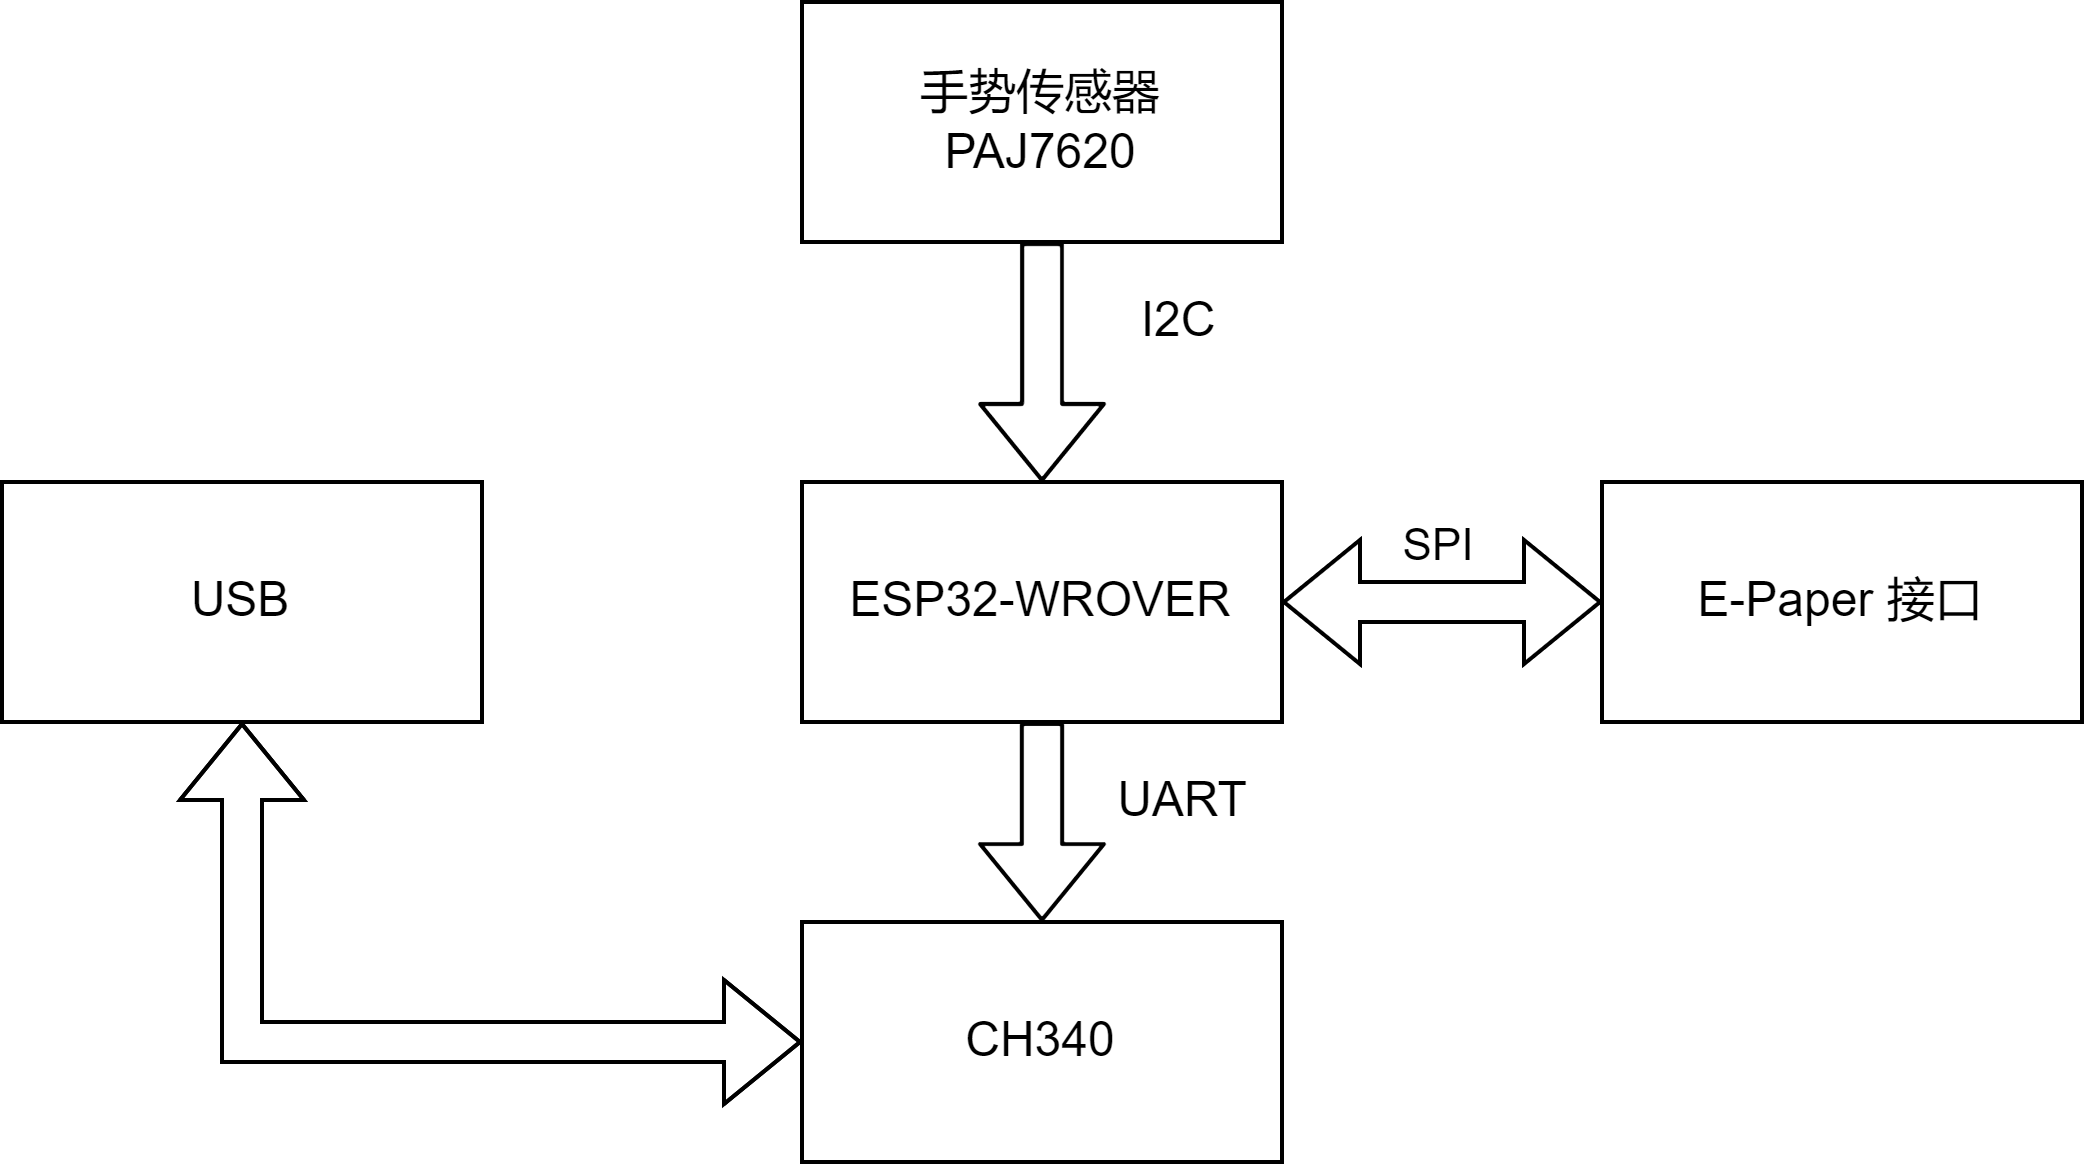
\includegraphics[width=.8\linewidth]{架构.drawio.png}
        \caption{硬件架构图}
    \end{figure}
\end{frame}

\begin{frame}{硬件设计}
    \begin{figure}[htp]
      \centering
      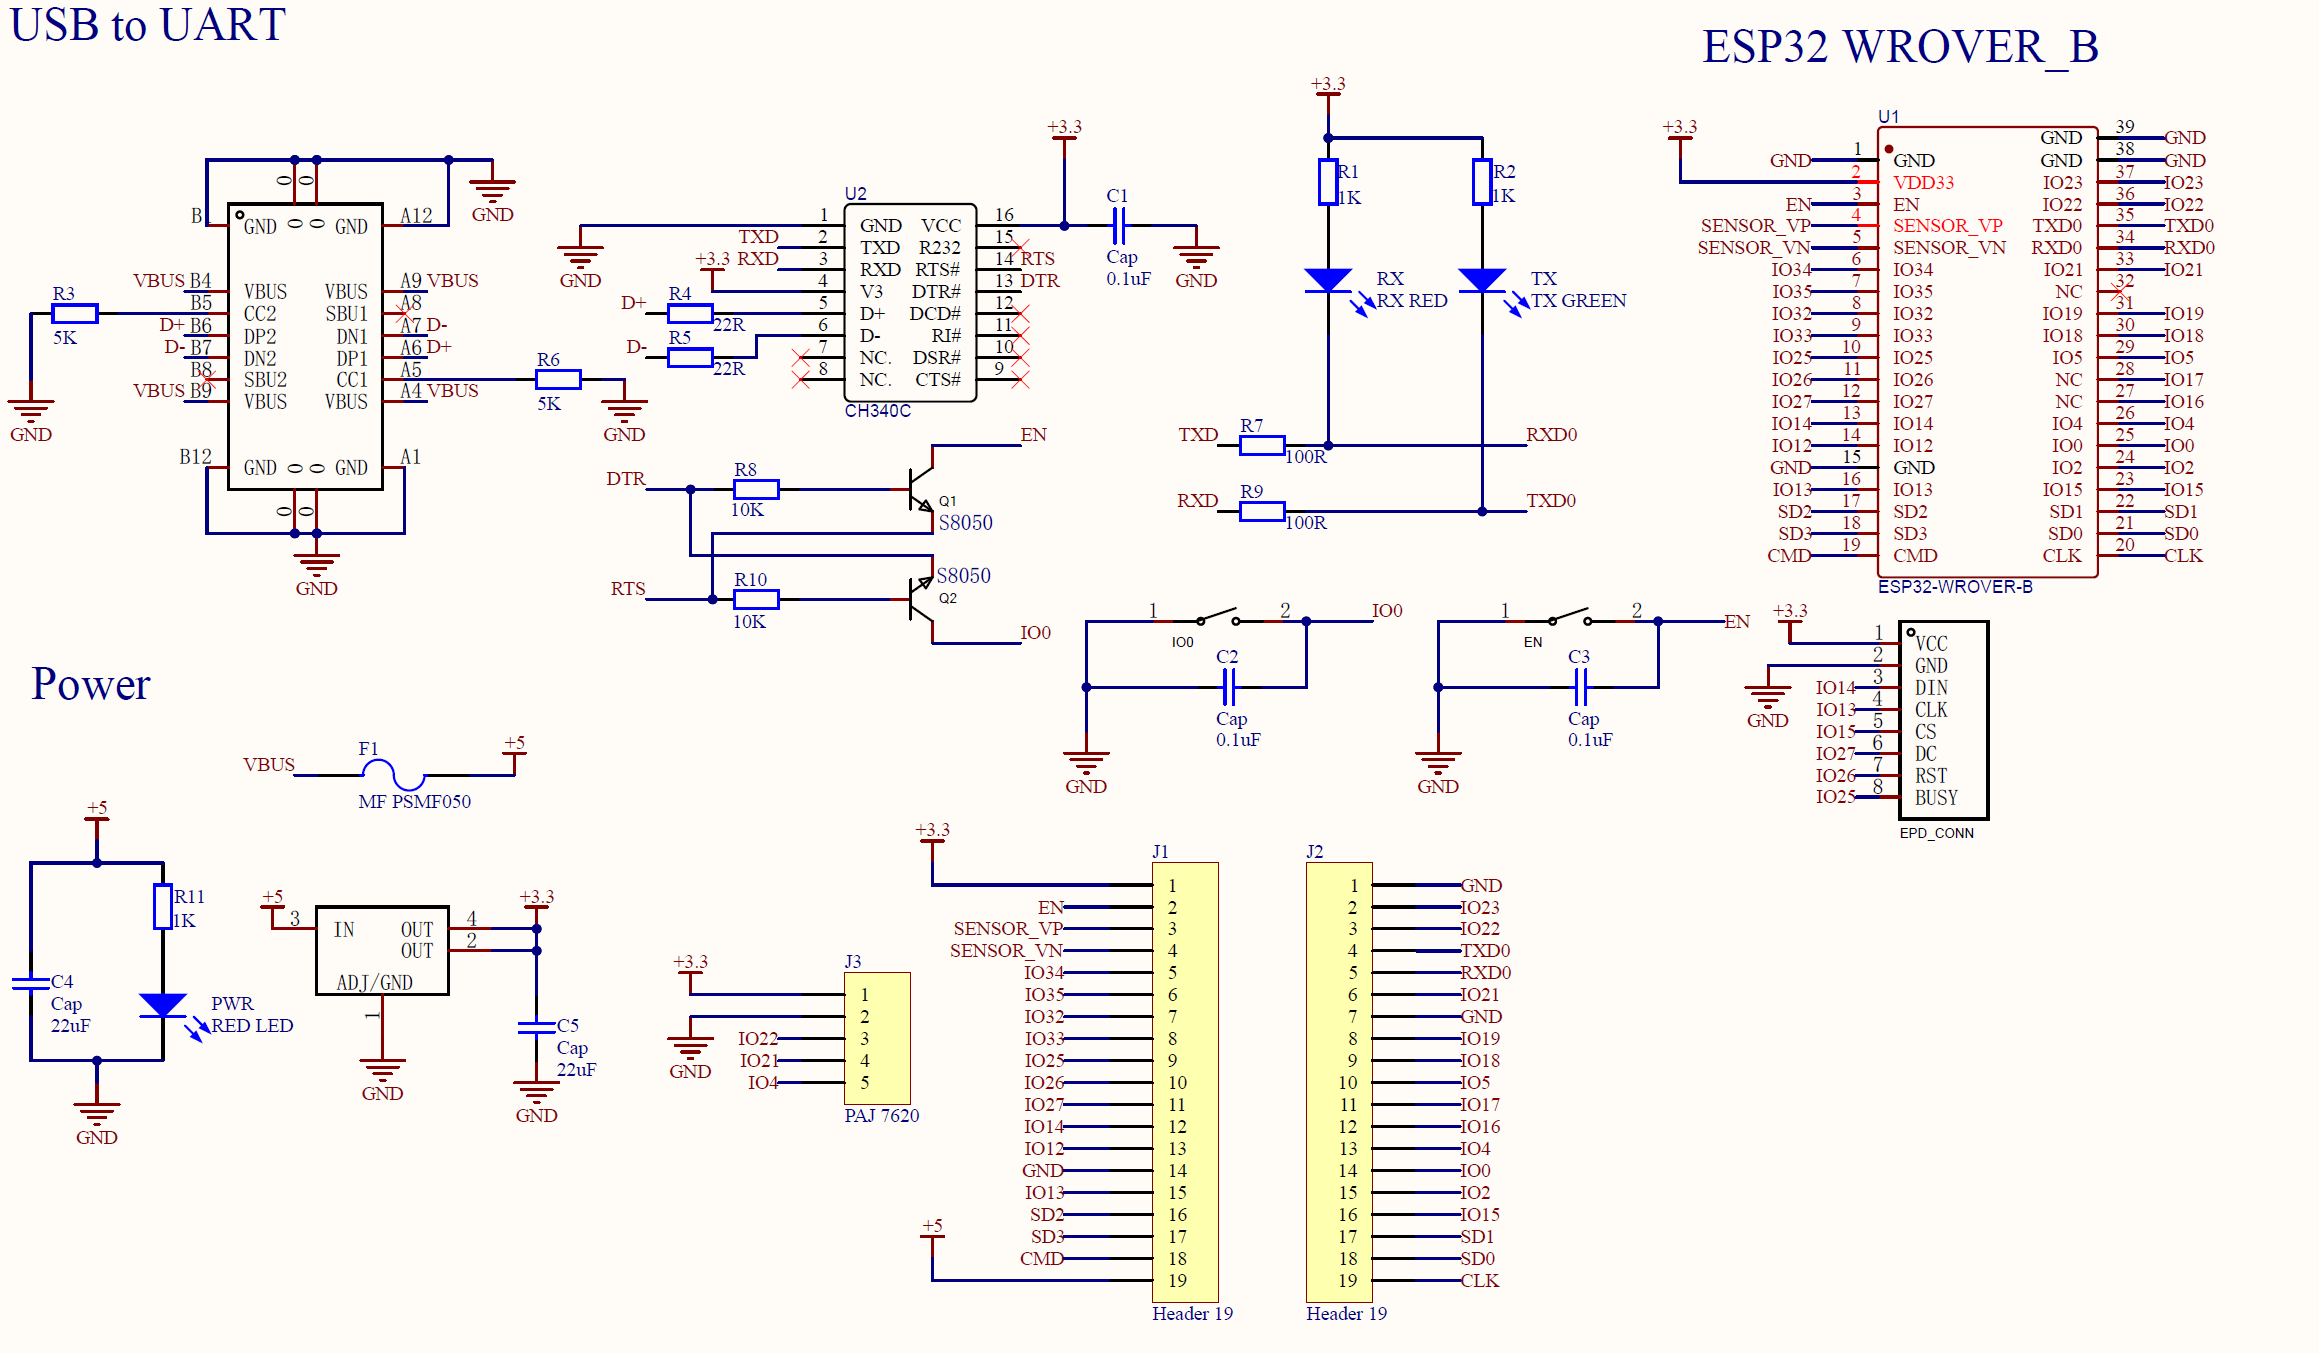
\includegraphics[width=\linewidth]{image5.png}
      \caption{原理图}
    \end{figure}
\end{frame}

\begin{frame}{硬件设计}
    \begin{figure}[htp]
      \centering
      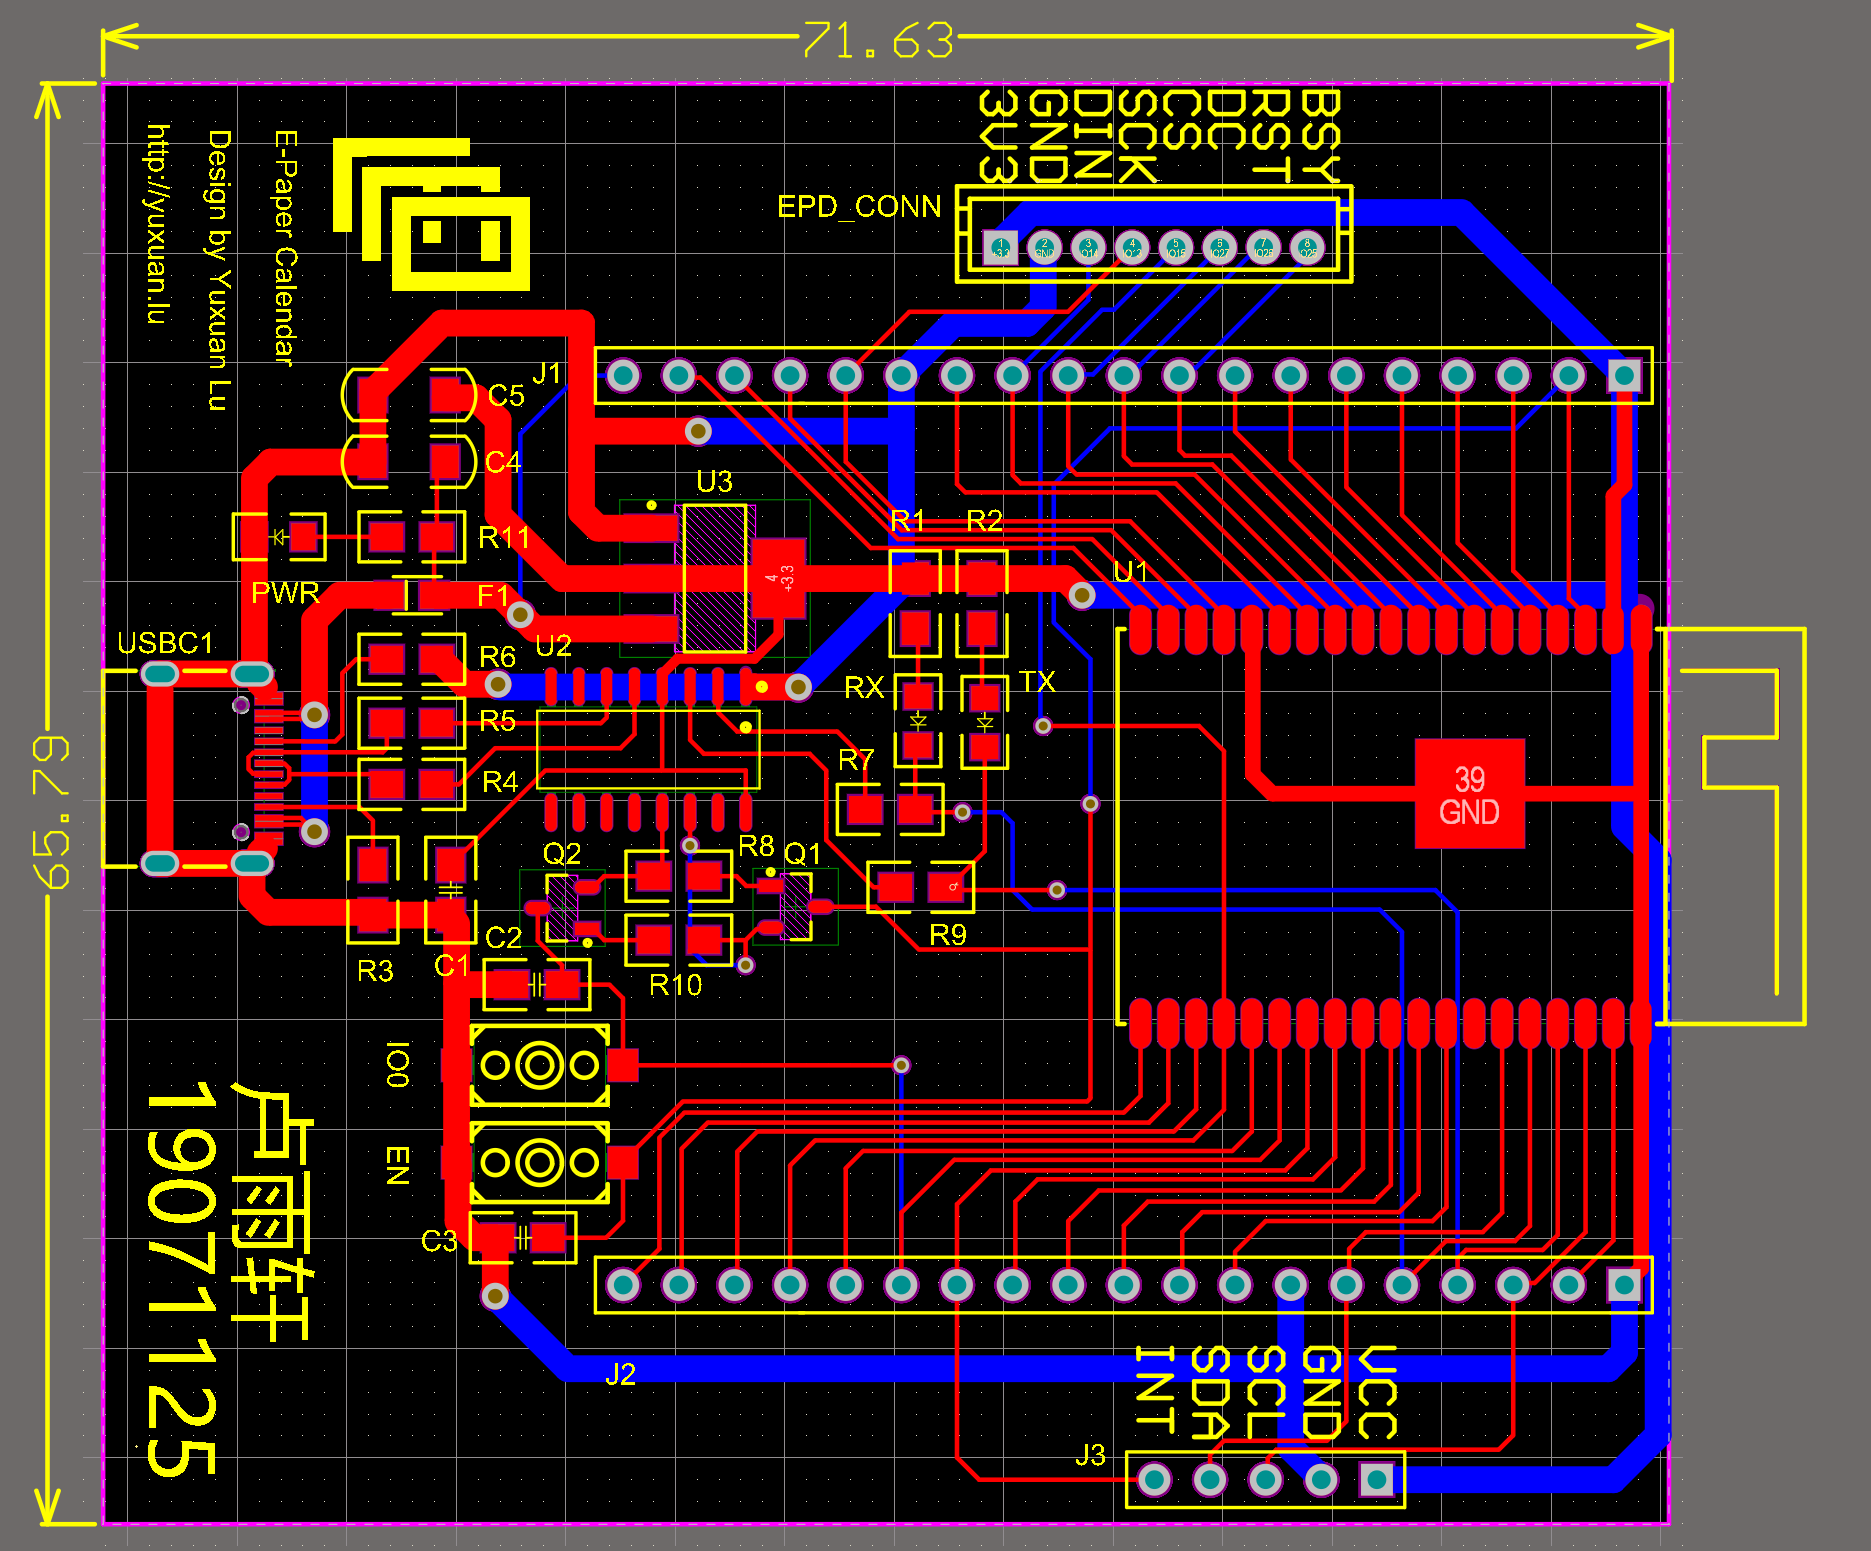
\includegraphics[width=.8\linewidth]{image6.png}
      \caption{PCB}
    \end{figure}
\end{frame}

\section{软件}

\begin{frame}{总体逻辑}
    \begin{figure}[htp]
      \centering
      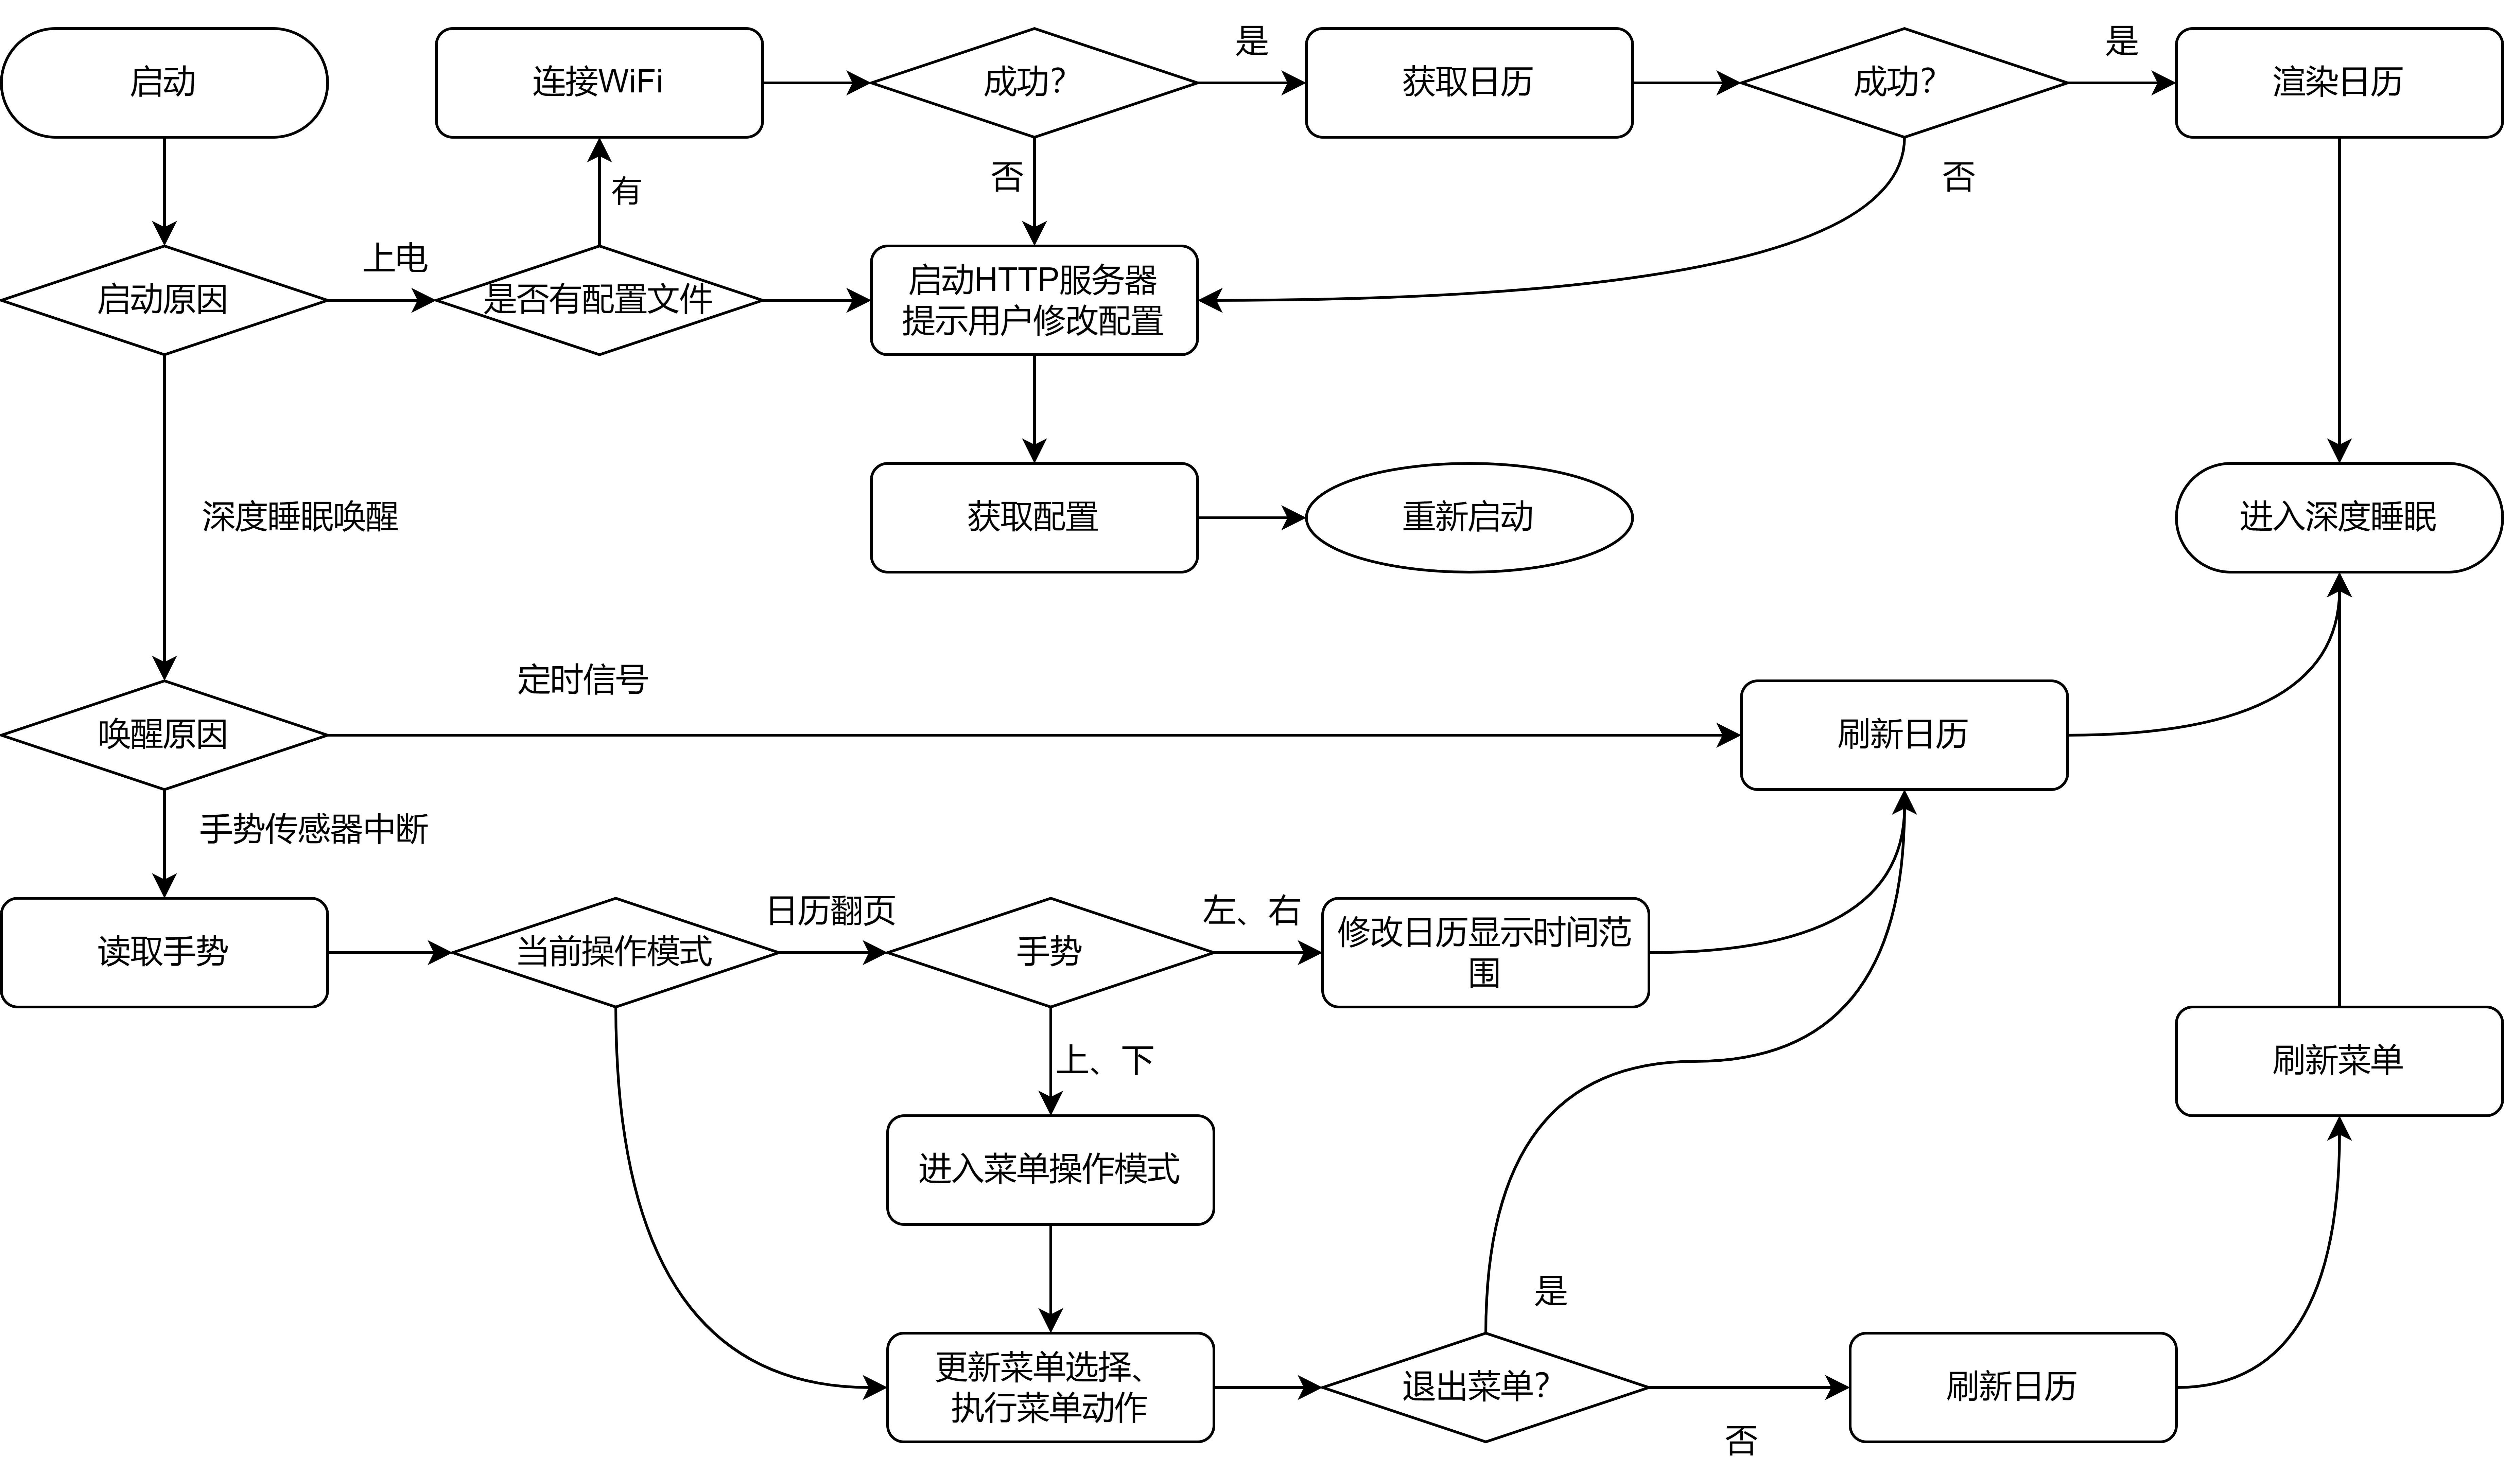
\includegraphics[width=.8\linewidth]{软件流程图.drawio.png}
      \caption{总体流程图}
    \end{figure}
\end{frame}

\begin{frame}{冷启动逻辑}
    \begin{outline}
        \1 第一次启动需要获取配置信息
            \2 WiFi 配置
            \2 日历订阅地址
        \1 如果没有发现配置信息(冷启动、恢复出场设置),则进入冷启动逻辑
            \2 开启热点
            \2 开启 http 服务器
            \2 提示用户连接热点,进入网页填写配置
        \1 接收到配置信息后,写入flash,并重启,进入正常启动逻辑
    \end{outline}
\end{frame}

\begin{frame}{冷启动逻辑}
    \begin{figure}[htp]
      \centering
      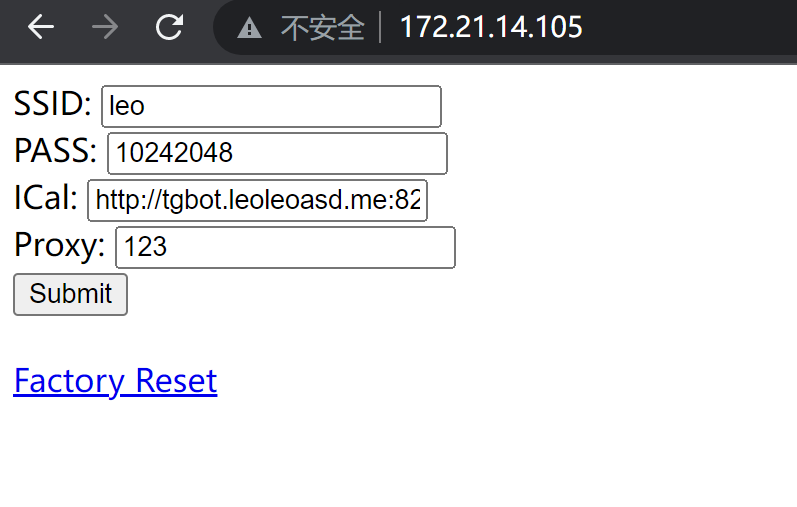
\includegraphics[width=.8\linewidth]{image7.png}
      \caption{http 配置界面}
    \end{figure}
\end{frame}
\begin{frame}{正常启动逻辑}
    \begin{outline}[enumerate]
        \1 初始化各个部分
            \2 flash、网络协议栈、外设
        \1 连接Wi-Fi
            \2 如果失败,清除flash中Wi-Fi设置后重启
            \2 进入冷启动逻辑
        \1 获取时间、获取日期
            \2 如果日历配置不存在,开启http 服务器,提示用户输入
        \1 将日历写入flash中
        \1 渲染日历
        \1 进入DeepSleep
            \2 唤醒条件:手势传感器中断或定时15分钟
    \end{outline}
\end{frame}
\begin{frame}{Deep Sleep 唤醒逻辑}
    \begin{outline}[enumerate]
        \1 如果是手势传感器中断:
            \2 进入手势传感器逻辑
        \1 如果是定时器中断:  
            \2 获取当前时间、刷新日历
            \2 目的:刷新日历上『当前时间』部分。
            \2 同时,用户可能翻页到下一页后忘了翻回来
                \3 定时15分钟回到默认状态
    \end{outline}
\end{frame}
\begin{frame}{手势传感器逻辑}
    \begin{outline}
        \1 如果当前模式为日历翻页
            \2 如果是上下,显示根菜单,进入菜单操作模式
            \2 如果是左右,日历左右翻页
        \1 如果当前模式为菜单操作
            \2 传递操作给菜单组件
            \2 如果退出根菜单,则回到日历翻页模式
    \end{outline}
\end{frame}
\begin{frame}{菜单组件设计}
    \begin{outline}
        \1 难点
            \2 任意级别菜单,结构复杂
            \2 需要跨deep sleep维护选择状态
                \3 可能有多层
        \1 实现:多层双向循环链表
    \end{outline}
\end{frame}
\begin{frame}{菜单组件设计}
    \begin{figure}[htp]
        \centering
        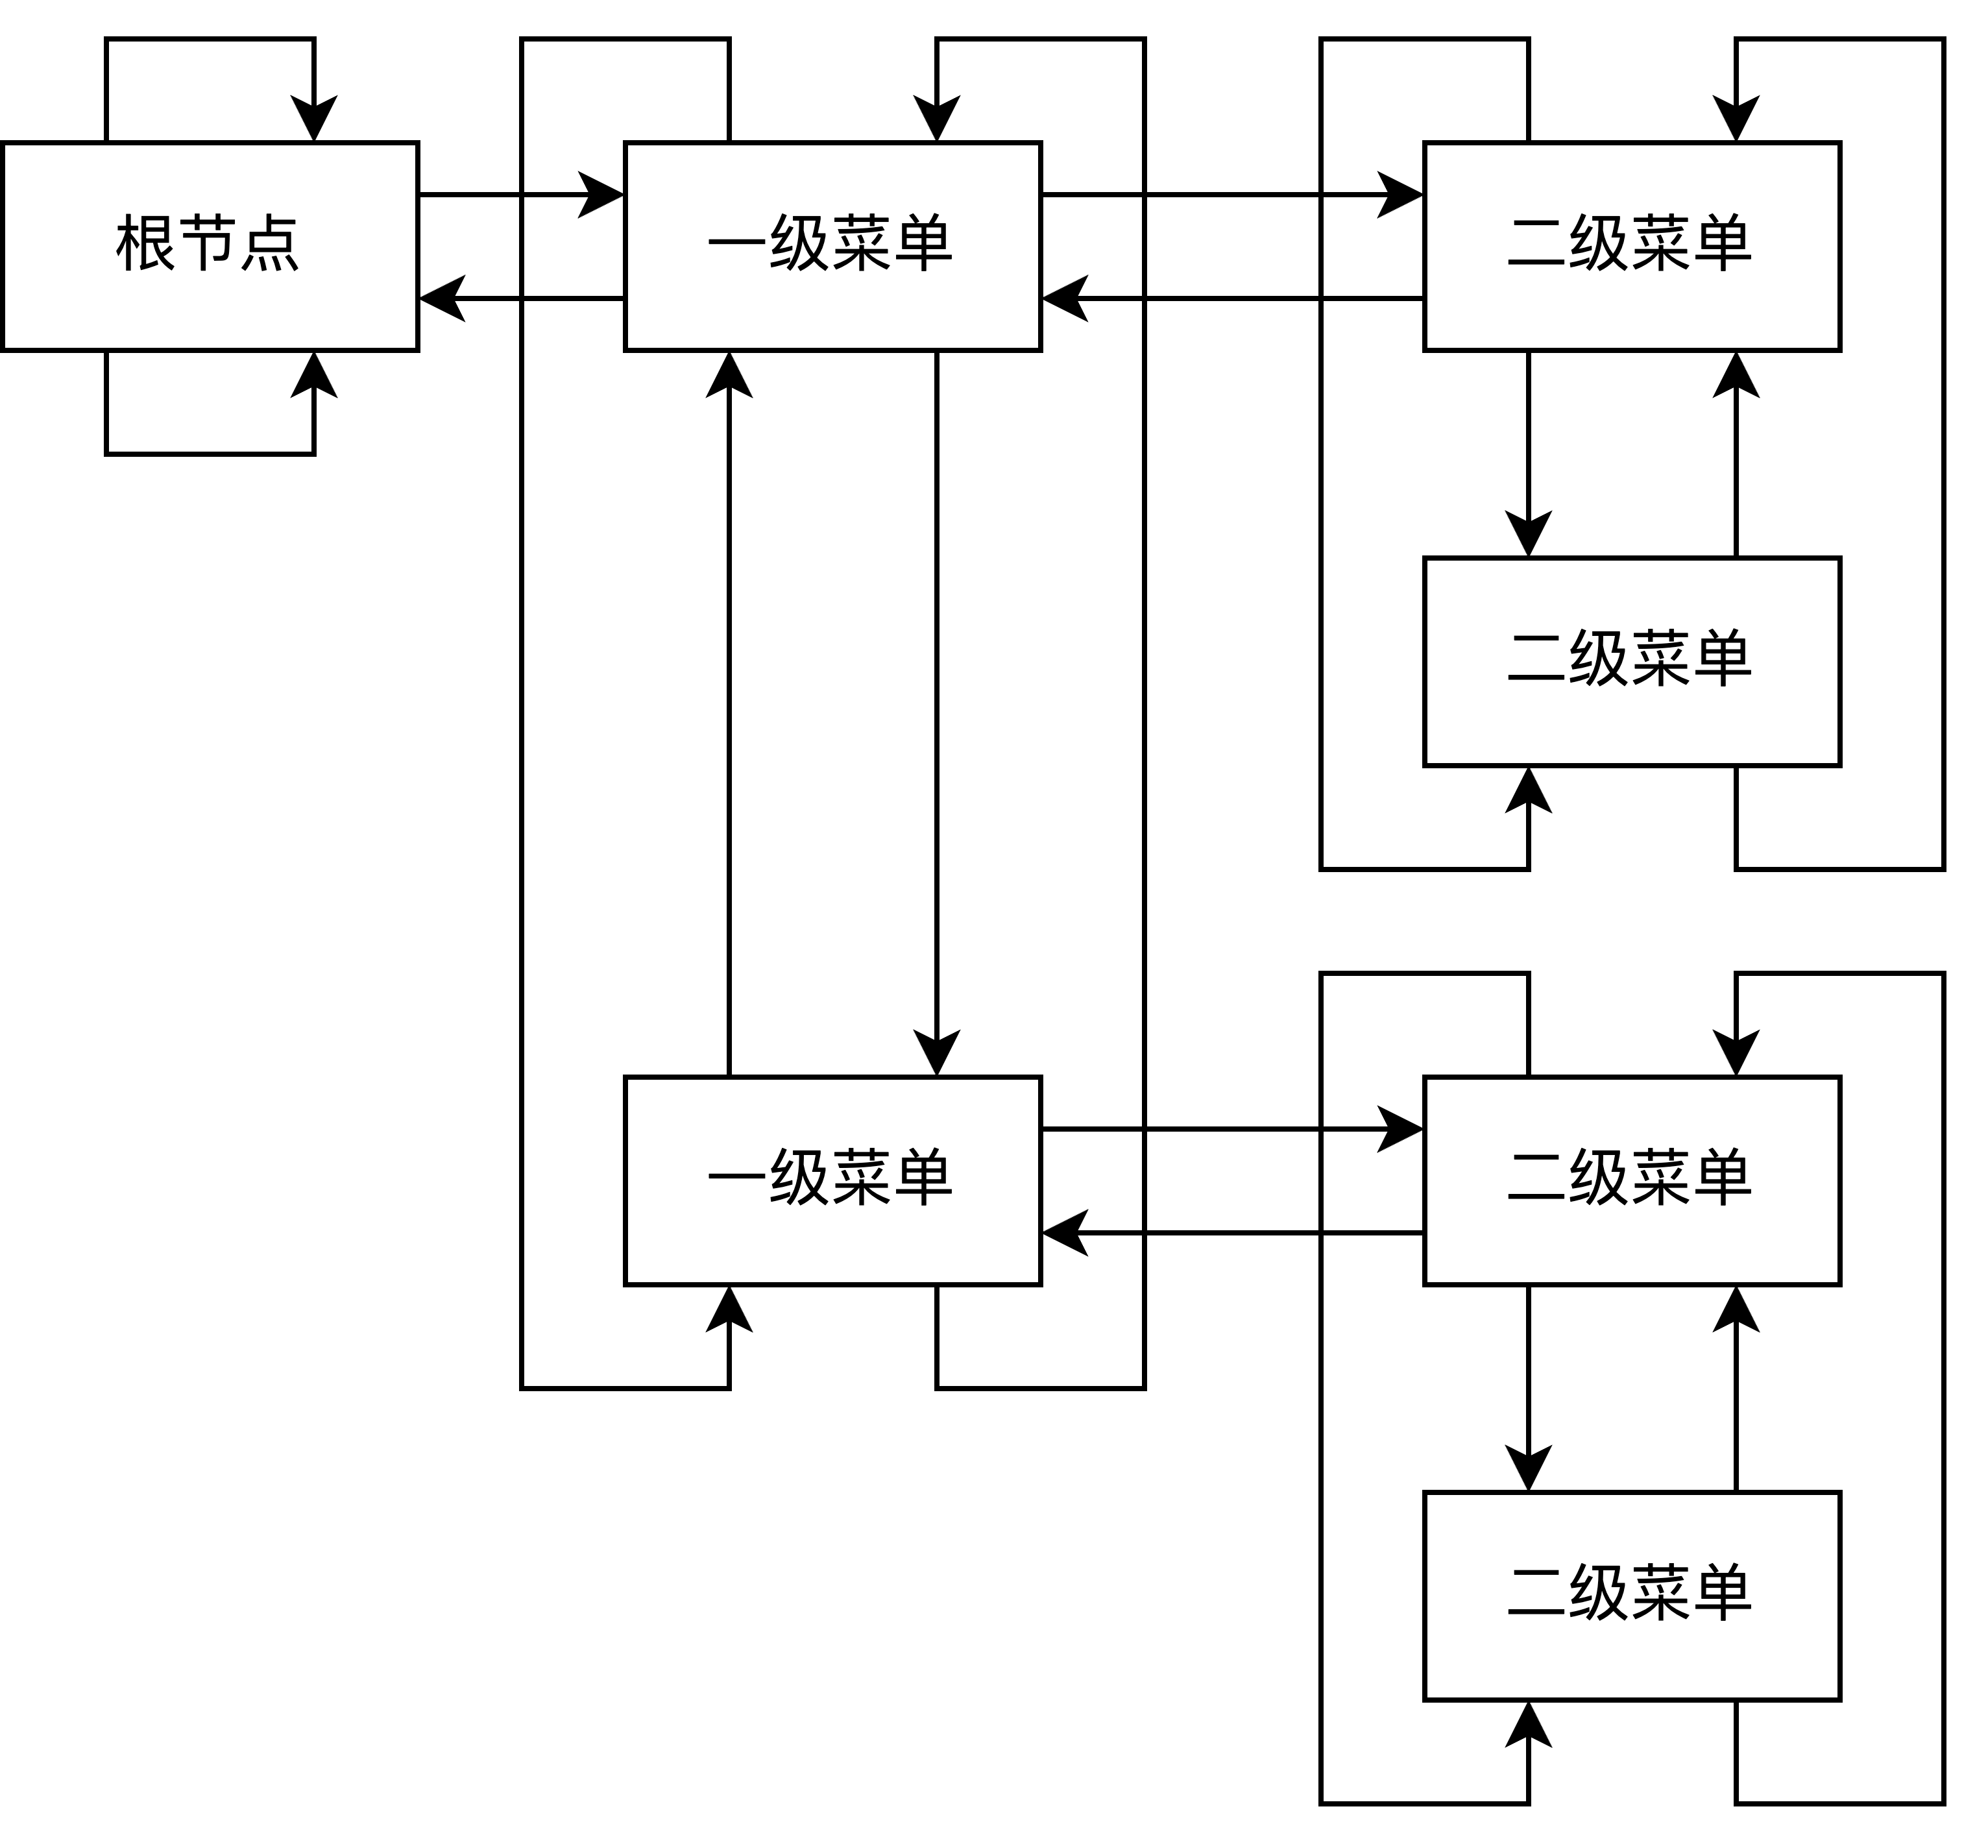
\includegraphics[width=.7\linewidth]{menu.drawio.png}
        \caption{菜单组件设计}
      \end{figure}
\end{frame}
\begin{frame}{菜单状态维护}
    \begin{outline}
        \1 难点:菜单是多层级的数据结构,难以放入RTC MEMORY
        \1 设计:
            \2 将所有菜单存入数组中,用下标访问
            \2 构建菜单的函数不变,则同一个菜单在数组中的下标不变
            \2 保存当前所在的菜单和选中的字菜单两个下标
            \2 2字节即可维护256个菜单的状态
    \end{outline}
\end{frame}
\section{总结}
\begin{frame}{总结}
    \begin{outline}
        \1 学习、熟悉、利用了各类硬件特性
            \2 WiFi、AP
            \2 Event Loop
            \2 FreeRTOS 特性
            \2 Deep Sleep
            \2 $\cdots$
        \1 在嵌入式场景下针对性设计解决方案
            \2 日历渲染
            \2 菜单渲染
            \2 菜单状态维护
        \1 不足
            \2 由于时间限制,没能引入完整电源管理
                \3 频率等
            
    \end{outline}
\end{frame}

\end{document}
